\section{Satellite multispectral imaging}
Satellite imagery have been employed for environmental monitoring purposes since the first satellite of NASA’s Landsat program started beaming back pictures in 1972 \cite{wang2007impact, williams2006landsat, 3320}.
This kind of imagery has numerous applications and makes a unique contribution to various domains.
For instance, in the field of agriculture, some crops occupy hundreds or even thousands of hectares, making it is nearly impossible for a farmer to efficiently monitor the state of its fields. Using satellite imagery, farmers can get feedback about several different properties of interest, such as the quality of its irrigation, fertilization, \etc \cite{agronomy10050641}.

To appropriately capture and analyze different properties of the environment, the satellites have to acquire the land at different bands of wavelengths, referred to as multi-spectral or hyper-spectral imaging.
Multi-spectral imaging is a term describing an acquisition of a certain scene in more than a single band of wavelengths\cite{sun2010hyperspectral}.
By this definition, some even consider the RGB camera as a multi-spectral camera, since the acquisition results in 3-channels of different (yet somewhat overlapping) bands of wavelengths. 
Generally speaking, multi-spectral imaging is used in applications where several bands of wavelengths are of interest, where each band provides different type of information about the scene, as illustrated in figure \ref{fig:multispectral}. 

\begin{figure}[H]
    \centering
    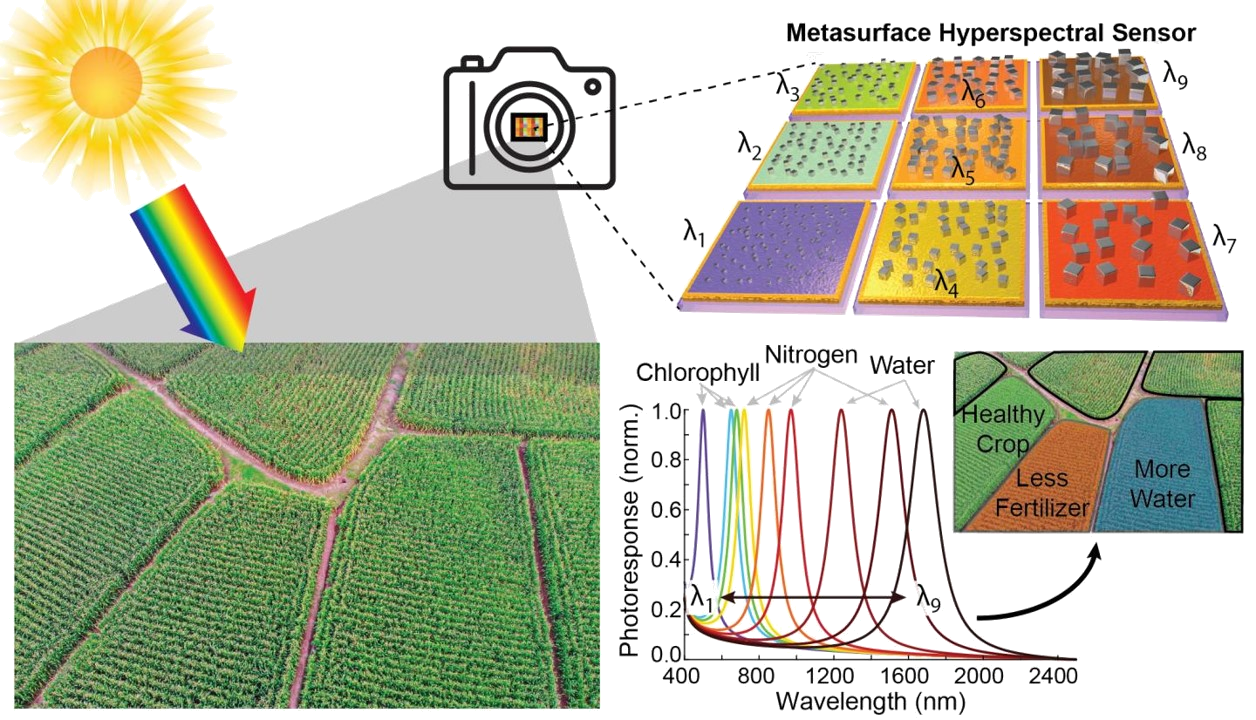
\includegraphics[width=\linewidth]{../figs/introduction/multispectral.png}    
    \caption{Multispectral imaging . Each band encodes a different sort of information about the same scene \cite{stewart2020ultrafast}.}
    \label{fig:multispectral}
\end{figure}

Modern satellites such as Sentinel-3 / Modis perform multi-spectral acquisition in a large number of spectral bands, spanning from the visible spectrum ($400-700nm$) going through NIR and SWIR (near and shortwave infrared respectively) and even longwave infrared (LWIR), spanning between $7-14\mu m$ \cite{ahmad2002p1}.
In this research, the focus will be on the LWIR band. 
LWIR channels are used for several environmental monitoring purposes, such as signatures of minerals that may be related to hydrothermal activity \cite{article_LWIR}.

\section{Motivation}
While multi-spectral satellite imagery is available today, it's typically acquired by normally-sized satellites equipped with state-of-the-art (SOTA) cameras, which naturally results in a very expensive product. 
As an alternative to the expensive multi-spectral solution, nano-satellites could be used to carry smaller and cheaper LWIR thermal cameras \cite{article}. 
Using a flock of nano-satellites, each equipped with a different IR filter, a multi-spectral cube can be obtained by applying registration (a well known computer-vision task) between overlapping images acquired by the different nano-satellites, as illustrated in figure \ref{fig:registration}.
\begin{figure}[H]
    \centering
    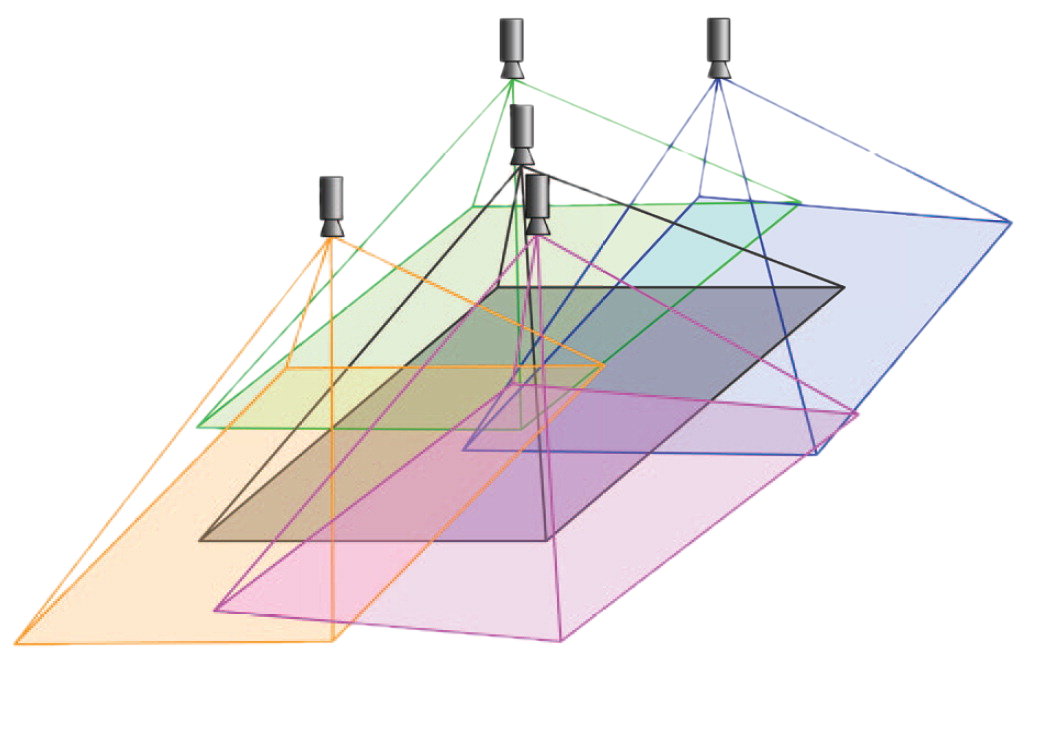
\includegraphics[width=\linewidth]{../figs/introduction/multicamera.png}
    \caption{Overlap between receptive fields of nano-sattellites, each equipped with a different IR filter.}
    \label{fig:registration}
\end{figure}

To generate a multi-spectral cube using a flock of nano-satellites, a dedicated multi-spectral registration algorithm must be developed.
However, both the training and validation stages of such an algorithm heavily depend on the availability of multi-spectral data.
Furthermore, this data should contain overlapping scenes across different spectral channels, and be compatible with the type of camera and filters that will eventually be mounted on the nano-satellites. 
While there is an abundance of panchromatic (wide banded) thermal aerial images, there is no available set of overlapping monochromatic (narrow band) thermal images. 
However, this caveat could be mitigated to some extent if overlapping monochromatic images could be generated artificially.
Hereby, we wish to construct a simulator that can generate a monochromatic image that's conditioned on the content of a panchromatic image. 
The artificially produced images of such a simulator could be used to develop the desired multi-spectral registration algorithm, which in turn will help increase the confidence in utilizing the concept of the nano-satellites flock for the thermal regime.

\section{Research scope and contribution}
Image to image (I2I) translation is the task of transforming the style of an image to that of a different domain while preserving its content. 
In many cases, there are no pairs of content-equivalent images in the input and output domains, \eg, there is no real image of a horse that is content-wise identical to a real image of a zebra. 
The I2I transformation in those cases is termed \emph{unpaired}.
Many methods have been developed to tackle this task, utilizing various deep neural architectures such as auto-encoders \cite{zhao2021unpaired}, generative adversarial networks (GANs) \cite{CycleGAN2017, park2020cut, zhao2020unpaired}, diffusion models \cite{DBLP:journals/corr/abs-2104-05358, saharia2022palette} and more.
Those methods have countless applications and are being used for numerous purposes, such as synthetic dataset generation for learning tasks in fields like autonomous cars \cite{https://doi.org/10.48550/arxiv.1812.01710, Dundar2018DomainSA}, medical imaging \cite{Thambawita_2022, chen2021synthetic}, \etc.
As the unpaired image-to-image (UI2I) translation task is unsupervised and highly ill-posed, those models are usually very hard to train.
Even when the produced outputs are visually appealing, it is not clear how authentic they are due to the inherent lack of ground truth.

What if our domains of interest had unique underlying physical properties that contain some additional information on the expected output?
The field of longwave-infrared (LWIR) imaging, \aka thermal imaging, enjoys such unique physical properties.
These properties enable the design of closed-form transformations between thermal modalities, which can be embedded in deep UI2I architectures to improve their performance.

To test this novel hypothesis, we first train two different SOTA GANs for UI2I translation between two thermal modalities to establish a baseline.
We then provide the generators with an additional physical property of the acquired images, allowing the GANs generator's output to be conditioned on that property.
Finally, we design a physical estimator and fuse it with the generator, resulting in our proposed method, named a physically enhanced thermal image-translating (PETIT) GAN.

Statistical analysis showed that our solution achieves an improvement of approximately $50\%$ compared to the SOTA GANs \wrt the conventional evaluation metrics.
Furthermore, our method exhibits a more consistent training procedure, possibly indicating convergence to flatter minima.
These improvements are further demonstrated qualitatively through our method's greater fidelity to the desired target domain.

\section{Thesis structure}
The remainder of this thesis is organized as follows: 
\begin{enumerate}
    \item Chapter \ref{sec:literature_review} introduces relevant background and theory, as well as prominent papers, upon which the method developed in the thesis is based. 
    Most of the content included in this chapter revolves around deep artificial neural networks and more concretely generative adverserial networks.
    \item Chapter \ref{sec:methods} presents the proposed method for applying deep thermal image to image translation using a physical estimator. The chapter includes details about the physical estimator, the calibration of its parameters, the architecture of the deep generative network and the fusion of the deep network with the physical estimator.
    \item Chapter \ref{sec:data} describes the procedure of the data collection and the preprocessing steps that were applied to prepare the data for training and evaluating the proposed method.
    \item Chapter \ref{sec:experiments} exhibits an evaluation the method and its different variants, and compares it to state of the art models. The comparison is made both quantitatively and qualitatively.
    \item Chapter \ref{sec:conclusions} summarizes and discusses the main results and provides possible directions for future work.
\end{enumerate}




